\documentclass[12]{report}
%\usepackage[utf8]{inputenc}
\usepackage{graphicx}
\usepackage{appendix}
\usepackage[a4paper,width=150mm,top=25mm,bottom=25mm,bindingoffset=6mm]{geometry}
\graphicspath{{photos/}}
\usepackage{caption}
\usepackage{enumitem}
\usepackage{blindtext}
\usepackage{algorithmic}
\usepackage{algorithm2e}

%\usepackage[latin1]{inputenc}
\usepackage[T1]{fontenc}
\usepackage[english]{babel}




\usepackage{xcolor}
\usepackage{listings}
\definecolor{mGreen}{rgb}{0,0.6,0}
\definecolor{mGray}{rgb}{0.5,0.5,0.5}
\definecolor{mPurple}{rgb}{0.58,0,0.82}
\definecolor{backgroundColour}{rgb}{0.95,0.95,0.92}

\lstdefinestyle{CStyle}{
	backgroundcolor=\color{backgroundColour},   
	commentstyle=\color{mGreen},
	keywordstyle=\color{magenta},
	numberstyle=\tiny\color{mGray},
	stringstyle=\color{mPurple},
	basicstyle=\footnotesize,
	breakatwhitespace=false,         
	breaklines=true,                 
	captionpos=b,                    
	keepspaces=true,                 
	numbers=left,                    
	numbersep=5pt,                  
	showspaces=false,                
	showstringspaces=false,
	showtabs=false,                  
	tabsize=2,
	language=C
}







\newcommand\tab[1][1cm]{\hspace*{#1}}



\usepackage{biblatex}
\addbibresource{ref/references.bib}

\begin{document}

	
%%%%%%%%%%%%%%%%%%%%%%% Title page %%%%%%%%%%%%%%%%%%%%%%%%%%%%%%%%%%
\begin{titlepage}%   
\vspace*{-3mm}

%%\begin{figure*}
%%\centering
%%\includegraphics[width=0.3\linewidth]{logo-univ.png}
%%\label{fig_logos}
%%\end{figure*}

\vspace*{-3mm}

%\begin{flushleft}
%{Num\'ero d'ordre: ***** \hfill Ann\'ee 2016}\par
%\end{flushleft}

\vspace*{-1mm}

\begin{center}% 

{\large \scshape{Hassiba  Benbouali University of Chlef}}\\
\vspace*{2mm}
{\large \scshape{Faculty of Exact Sciences and Computer Sciences}}\\
\vspace*{2mm}
{\large \scshape{Departement of Computer Sciences}}\par
\vspace*{2mm}\vspace*{0.8cm}
{\large  \scshape{Graduation project
For Obtaining the Bachelor degree}}\par
\vspace*{2mm}\vspace*{0.5cm}

{\large Submitted by}\\
\vspace*{3mm}
{\large Seyyidahmed Lahmer $\&\&$   Kheroubi Elaid  }\\
\vspace*{0.5cm}
\rule{150mm}{.75pt}\par%
\vspace*{5mm}%
\newbox\titlebox%
{\scalebox{1}[1]
{\hspace{-0.75cm}\parbox{165mm}
%\leftmargin \leftmarginv
{\huge\centering\scshape{  Synchronisation in wireless sensor network }}}}\par
\vspace*{5mm}
\rule{150mm}{.75pt}%\par
\vskip 2em

{ defended on (07/05/2018) in accordance with decision of following committee members:  }\\
%\vspace*{3mm}%
\vspace*{6mm}
%\vspace*{4cm}
\end{center}\par

\hspace{-1cm}\begin{tabular}{llcl}
 \hspace{5.5cm}	\textit{ Supervised  by:}\\	%&--& Maitre de Conf\'erences \`{a} l'Universit\'e de ???????????\\
	\hspace{6cm}	 Saiah Amin%&--& Maitre de Conf\'erences \`{a} ???????????\\
	   
		%&--& Maitre de Conf\'erences \`{a} l'Universit\'e de Chlef\\
\end{tabular}

\begin{flushleft}
%{Num\'ero d'ordre: *****
\vspace{2cm}
\centering
{ college year 2017/2018}\par
\end{flushleft}

%\vspace*{1.5cm}
%\begin{center}
%{Laboratoire d'InfoRmatique en Image et Syst\`emes d'information}\\
%{UMR 5205 CNRS - Lyon 1 - B\^at. Nautibus}\\
%{69622 Villeurbanne cedex - France}\\

%\end{center}
\end{titlepage}

\thispagestyle{empty}

%%% Local Variables: 
%%% mode: latex
%%% TeX-master: "manuscrit_these"
%%% End: 

	
	\chapter*{Didication1}	
	\chapter*{Didication2}
	\chapter*{Acknowledgments}
	
I would like to thank my Lord for giving me the opportunity and skill with which to write this Report,and Letting me see it to completion. I would like to thank my mother for countless cups of coffee ,good council and lots of patience, and for her Encouragement and prayer. I would like to thank my father for the hope and love, and for his encouragement and prayer. I would like to thank my to brothers( $Dr.Ilyes$ , Mohammed ) . i would thank my project supervisor Dr.Amin Saiah ,Without his assistance and dedicated involvement in every step throughout the process, this project would have never been accomplished. I would like to thank you very much for your support and understanding over these past months ,I would Like to thank my jury professors Dr NAME1  and Dr NAME . i would also like to thank my best college-mate ( Mohammed Elhouari , Sbaihia Nassim ,,, Koceir Lokman , Madani abderahmane , Kella youssouf , Kerfa abdelhamid , bouhraoua abdellah) . I would also thank all my teachers espacially Dr.Mohamed Slimane,Dr.Mohammed Amin Tahraoui and Dr.Ahmed Slimani  and our department responsable Dr. Toufik Taalibi BOUKERCHE .Finally i would thank everybody else .

	
	
	\chapter*{Terminology}
	\begin{itemize}
	\item \textbf{WSN} Wireless Sensor Network
	\item \textbf{CMTS} Consensus-based Multi-hop Time Synchronization
	\item \textbf{MLEs} Maximum Likelihood Estimation
	\item \textbf{GPS} Global Positioning System 
	\item \textbf{RBS} Reference Broadcast Synchronization
	\item \textbf{DMTS}  Delay Measurement Time Synchronization
	\item \textbf{FTSP}  Flooding Time Synchronization Protocol
	\item \textbf{MAC}  Medium Access Control 
	\item \textbf{OSI}  Open System Interconnection
	\item \textbf{QOS} Quality Of Service
	\item \textbf{ROS} Receiver Only Synchronization 
	\item \textbf{} 
	\item \textbf{} 
	\item \textbf{} 
	\item \textbf{} 
	\item \textbf{} 
	\item \textbf{} 
	\item \textbf{} 
	\item \textbf{} 
	\item \textbf{} 

\end{itemize}
	

	
	\tableofcontents
	
	
	\listoffigures

	


	
	\chapter*{Introduction}
	\section{context of the project}
In recent years,  wireless  sensor network,has received much attention  of  researchers,One of the main pervasive problems WSN
encounter is  to maintain  flawless communication sharing  and  cooperative 
processing between sensors  via  radio  links to  ensure a  reliable  treatment  of 
information.Many  applications  based  on  these  WSNs consider local  clocks  at  each  sensor node  that  need  to  be  synchronized  to  a  common  notion  of  time.
In  this  context,the  majority  of  previous  researches were focused  on  the  study  of  protocols,  and algorithms   that   address   these issues   in   order   to   resolve  synchronization problems. Previous  fforts and empirical  studies  in WSN proposed several solutions (algorithms). 
The focus of this thesis is to implement a tiny-small C-library that helps motes to run operations that deals with big numbers .  
\section{problematic}	

\section{Objectifs}
The main objective of this project is to implement a small portable library written in C for arbitrary precision arithmetic on integers, rational numbers, and floating-point numbers.  It aims to provide the possible arithmetic for all applications that need higher precision,numbers than is directly supported by the basic C types.\\
Features : 
 \begin{itemize}
	\item Integers and decimals
	\item smaller perhaps Faster,easier to use than other c libraries(Lite Version)
	\item No dependencies
	\item No Dynamic Allocation
	\item Comprehensive documentation 

\end{itemize}

	
	
	\chapter{Wireless Sensor Network}
	\section{Introduction}
	Wireless sensor network \cite{wsn} is a popular area for research now days, due to vast potential usage of sensor networks in different areas.A sensor network is a comprised of sensing, processing, communication ability which helps to observe, instrument,react to events and phenomena in a specified environment \cite{wsn2} \cite{wsn3}.This kind of network  enables  to  connect  the  physical  world  to  environment.   By  networking
	tiny sensor nodes, it becomes easy to obtain the data about physical phenomena which was very much difficult with conventional ways.Wireless sensor network typically consist of tens to thousands of nodes. These nodes collect, process and cooperatively  pass  this  collected  information  to  a  central  location.   WSNs  have unique characteristics such as low duty cycle, power constraints and limited battery  life,  redundant  data acquisition,  heterogeneity  of  sensor  nodes,  mobility  of nodes,  and  dynamic  network  topology,  etc  \cite{wsn2}. 
\section{Application Of WSN}
	There are numerous applications of WSNs in Military, traffic monitoring and control, medical device monitoring and in many other areas. Some of applications are discussed below:
	\begin{figure}
	\subsection{Military or Border Surveillance Applications}
		WSNs are becoming an integral part of military command,control,communicatio and intelligence systems.Sensors can be deployed in a battle field to
		monitor the presence of forces and vehicles, and track their movements, enabling close surveillance of opposing forces  see \ref{fig:x army} .\cite{application}
	
	%Figure Army Application Right Here
	%	\begin{figure}[h!]
	%		\centering
	%		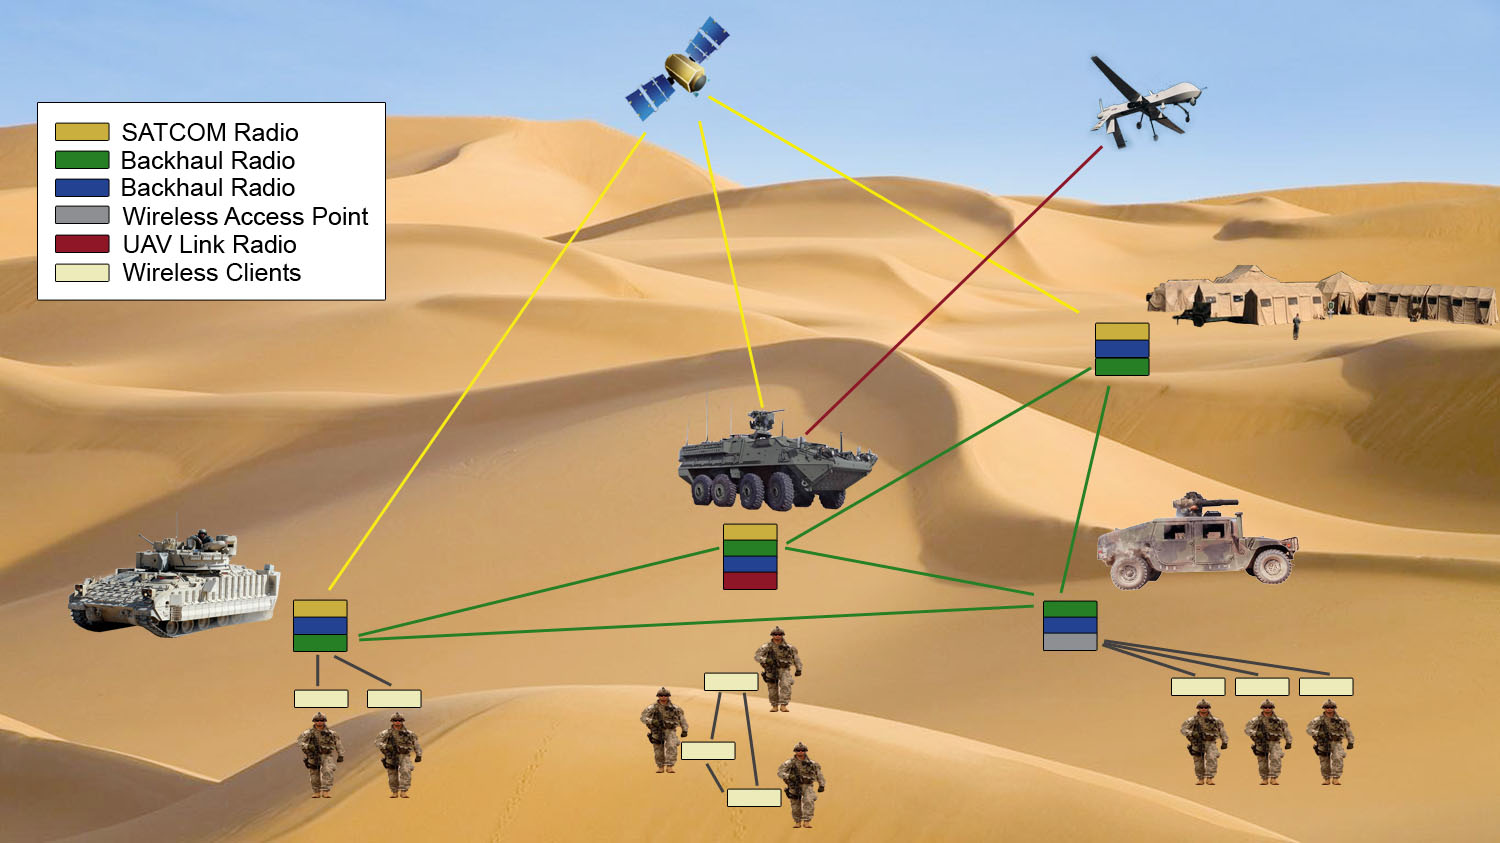
\includegraphics[scale=0.5,width=15cm,height=9cm]{photos/army.jpg}
	%		\caption{Military Surveillance App}
	%		\label{fig:x army}

	%	\end{figure}
	
	\hfill
	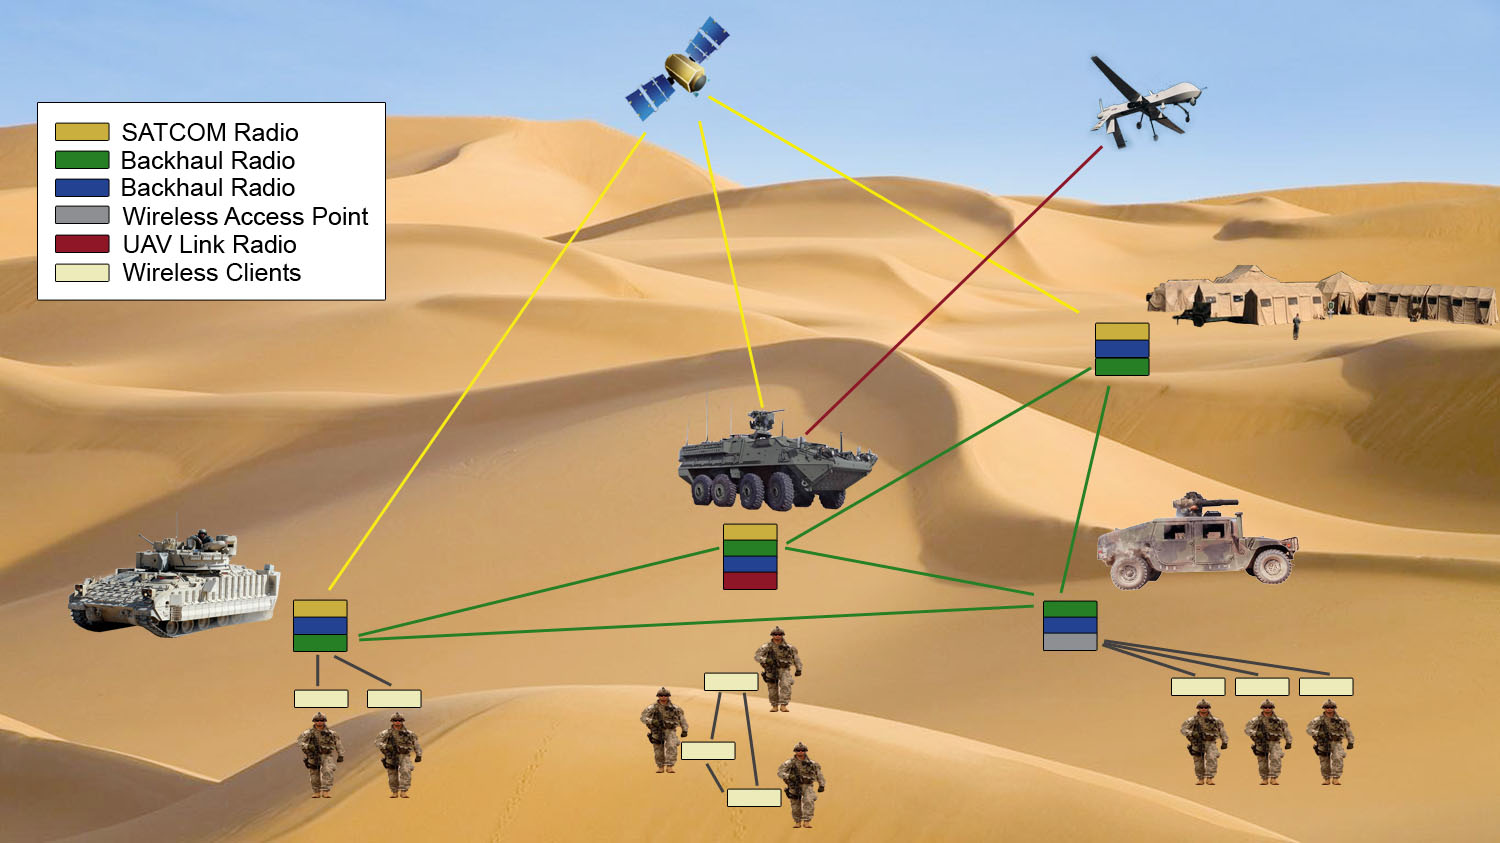
\includegraphics[scale=0.5,width=12cm,height=6.5cm]{photos/army.jpg}
	\caption{Military Surveillance App}
	\label{fig:x army}
		\centering
	\hspace*{\fill}
	\end{figure}

	\begin{figure}
	\subsection{Environmental Conditions Monitoring}
		 WSN applications in this area include monitoring the environmental conditions affecting crops or livestock,monitoring  temperature,  humidity  and lighting  in  office buildings, and so on. These monitoring modules could even be  combined  with  actuator modules which can control,for example , the amount of fertilizer in the soil, or the amount of cooling or heating in a building, based on distributed sensor measurements\cite{application} see\ref{fig:x Environmental_Conditions_Monitoring}.

	
	%Figure Env Condition Monitoring Right here
	%\begin{figure}[h!]
	%	\centering
	%	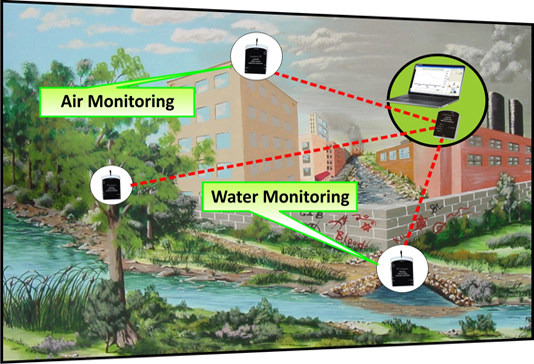
\includegraphics[scale=0.5,width=15cm,height=9cm]{photos/env.jpg}
	%	\caption{Environmental Conditions Monitoring}
	%	\label{fig:x Environmental_Conditions_Monitoring}	
	%\end{figure}

	
	\hfill
	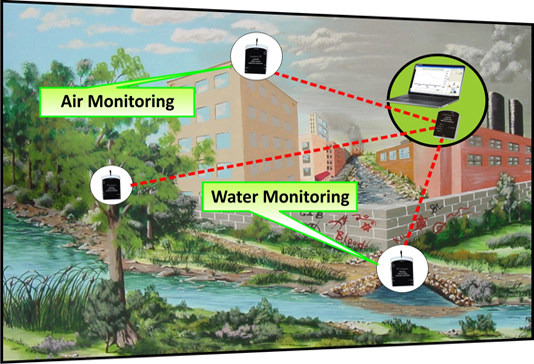
\includegraphics[scale=0.5,width=12cm,height=6.5cm]{photos/env.jpg}
	\caption{Environmental Conditions Monitoring}
		\centering
	\label{fig:x Environmental_Conditions_Monitoring}
	\hspace*{\fill}
 	\end{figure}

	\begin{figure}
	\subsection{Health Care Applications}
		Wireless  sensor  networks  can  be  used  to  monitor  and track  elders  and  patients  for  health  care  purposes,  which can significantly relieve the severe shortage of health care personnel  and  reduce  the  health  care  expenditures  in  the current  health  care  systems.  For  example  sensors  can  be deployed in a patient’s home to monitor the behaviors  of the patient. It can alert doctors when the patient falls and requires immediate medical attention\cite{application} see \ref{fig:x Health_Care_Applications}.
		
		
		
		\hfill
		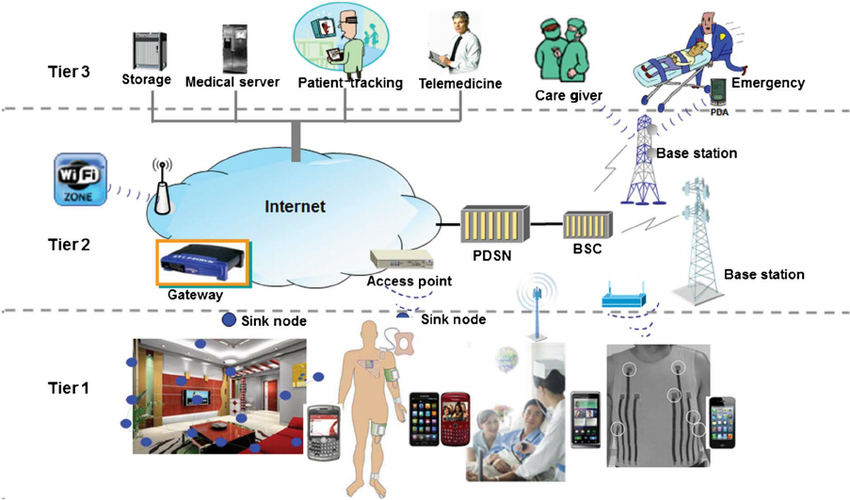
\includegraphics[scale=0.5,width=12cm,height=6.5cm]{photos/healthcare.png}
		\caption{Health Care Applications}
			\centering
		\label{fig:x Health_Care_Applications}
		\hspace*{\fill}
	\end{figure}
		
		%figure Health Care Application Right here
		%\begin{figure}[h!]
		%	\centering
		%	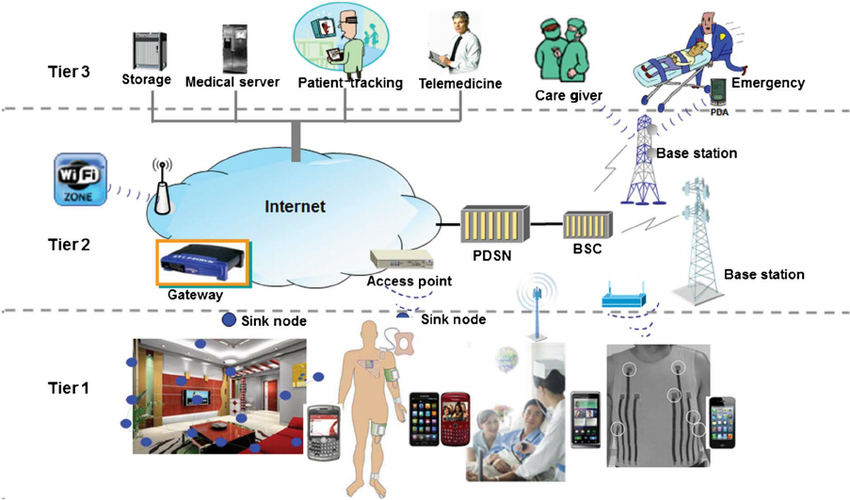
\includegraphics[scale=0.5,width=15cm,height=9cm]{photos/healthcare.png}
		%	\caption{Health Care Applications}
		%	\label{fig:x Health_Care_Applications}
			
		%\end{figure}
	
  \begin{figure}	
	\subsection{Home Intelligence}
			 Wireless sensor networks can be used to provide more convenient and intelligent living environments for human beings. For example, wireless sensors can be used to remotely read utility  meters in a home like water, gas, electricity and then  send  the  readings  to  a  remote  centre 
		through  wireless communication\cite{application} see\ref{fig:x Home_Intelligence}.
	
		\hfill
		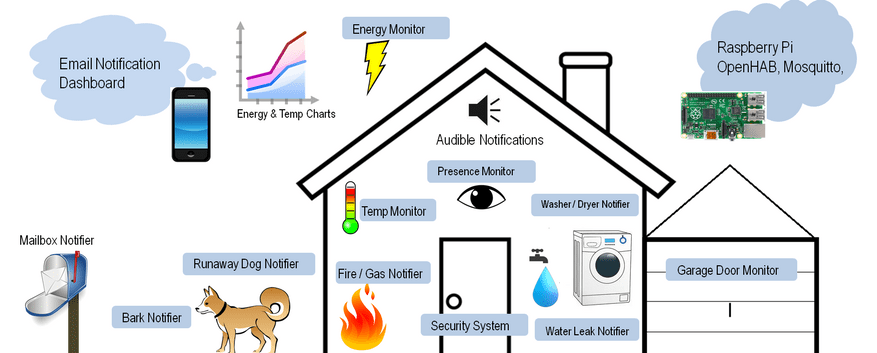
\includegraphics[scale=0.5,width=12cm,height=6.5cm]{photos/home.png}
		\caption{Home Intelligence}
		\label{fig:x Home_Intelligence}
			\centering
		\hspace*{\fill}
  \end{figure}
		  
    %figure Home Intelligence
   % \begin{figure}[h!]
    %	\centering
   % 	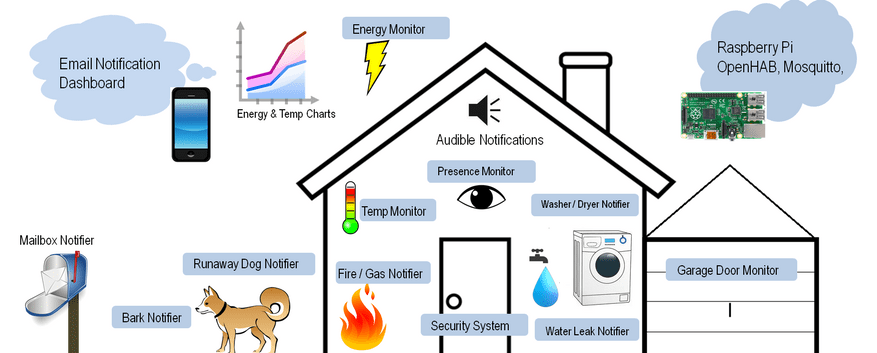
\includegraphics[scale=0.5,width=15cm,height=9cm]{photos/home.png}
    %	\caption{Home Intelligence}
    %	\label{fig:x Home_Intelligence}
    	
    % \end{figure}
    
   \begin{figure} 
    \subsection{Agriculture}
    
    Using wireless sensor networks within the agricultural industry  is  increasingly  common,  using  a  wireless  network frees the farmer from the maintenance of wiring in a difficult environment. Gravity  feed  water  systems  can  be  monitored using  pressure  transmitters  to  monitor  water  tank  levels, pumps can be controlled using wireless I/O devices and water use  can  be  measured  and  wirelessly  transmitted  back  to  a central  control  center  for  billing.  Irrigation  automation enables more efficient water use and reduces waste\cite{application} see\ref{fig:x Agriculture_}.
    
    %%figure Agriculture
	%\begin{figure}[h!]
	%	\centering
	%	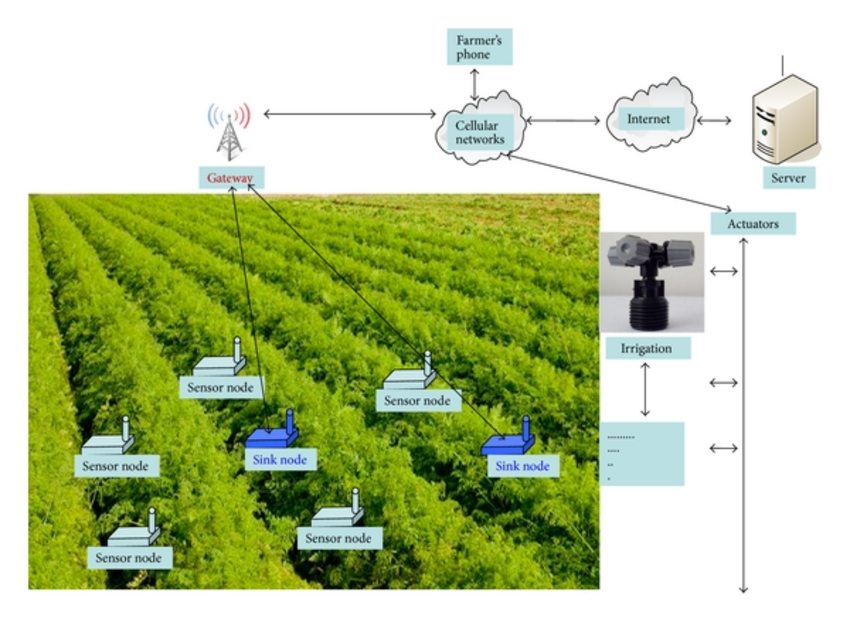
\includegraphics[scale=0.5,width=12cm,height=6cm]{photos/agri.png}
	%	\caption{Agriculture}
	%	\label{fig:x Agriculture_}
		
	%\end{figure}

	\hfill
	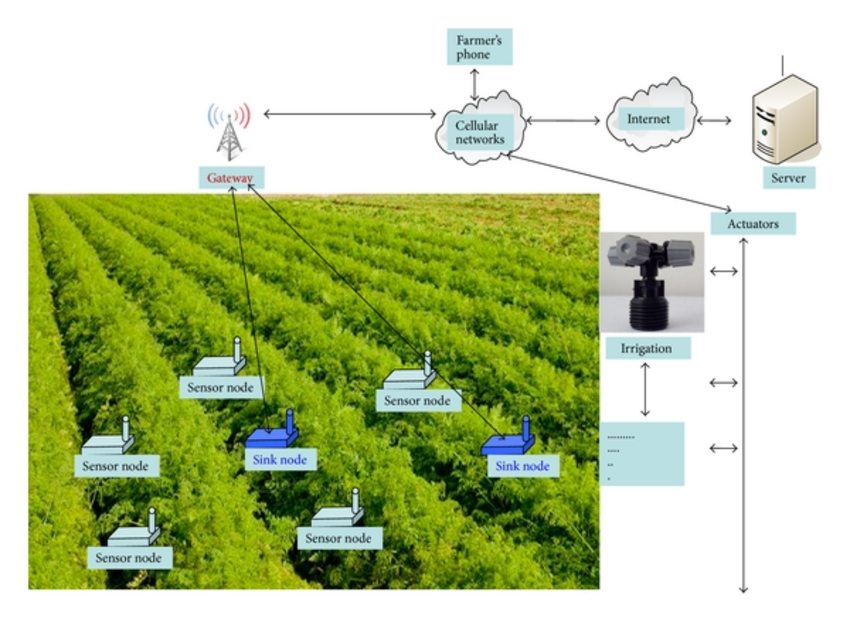
\includegraphics[scale=0.5,width=12cm,height=5cm]{photos/agri.png}
	\caption{Agriculture}
	\centering
	\label{fig:x Agriculture_}
	\hspace*{\fill}
\end{figure}
\section{Challenges}

Recent advances in technology has made researchers quite optimistic towards the feasibility of Wireless sensor networks (WSNs).  These are being deployed for various applications and have huge potential for research. However, owing to the multidisciplinary nature of this field, researchers have to face many a technical hitches,research issues and challenges involved in the design of WSNs\cite{resGateChallenges}. 
The major challenges that affect the design and performance of a wireless sensor network are as follows :
	\subsection{Energy}
	The first and  often most important design challenge for a WSN is energy efficiency.Power consumption  can  be  allocated  to  three  functional  domains: sensing, communication, and data processing, each of which requires  optimization.  The  sensor  node  lifetime  typically exhibits a  strong dependency on battery life. The constraint most  often  associated  with  sensor  network  design  is  that sensor nodes operate with limited energy budgets[ref.energy] \cite{energy}.  
	\newline
	Typically,  sensors  are  powered  through  batteries,which  must  be  either  replaced  or  recharged  when  depleted. For non rechargeable batteries, a sensor node should be able to  operate  until  either  its  mission  time  has  passed  or  the battery  can  be  replaced.  The  length  of  the  mission  time depends on the type of application\cite{energy}. 
	
	
	\subsection{Synchronization}
	Clock  synchronization is an important  service  in  sensor networks.Time Synchronization in a sensor network aims to provide a common timescale for local clocks of nodes  in  the  network.A global clock in a sensor  system  will  help  process and analyze the data  correctly and predict future system behavior.Some applications that require global clock synchronization are environment monitoring ,navigation guidance, vehicle tracking etc. A clock synchronization service for a sensor network has to meet challenges that are substantially different from those in infrastructure based networks\cite{sync2} \cite{sync1}
	
	
	
	\subsection{Security}
	Security in sensor networks is as much an important factor as performance    and    low    energy    consumption    in    many applications. Security in a sensor network is very challenging as WSN is not only being deployed in battlefield applications but  also  for  surveillance,  building  monitoring,  burglar  alarms  and in critical systems such as airports and hospitals\cite{}[Ref.security].
	Since  sensor  networks  are  still  a  developing  technology, researchers  and  developers  agree  that  their  efforts  should  be concentrated  in  developing  and  integrating  security  from  the  initial phases of sensor applications development; by doing so,they hope to provide a stronger and complete protection against illegal  activities  and  maintain  stability  of  the  systems  at  the  same time\cite{}.
	
	
	
	\subsection{Quality Of Service}
	WSNs are   becoming   more widely  deployed  for  real-world  monitoring, event detection,and target tracking  [e.g., \cite{}Ref.Qos]. Many of these applications require the  WSN  to  operate  autonomously in dynamic environmental settings, with desirable quality of service (QoS) where  the  control  is  adaptive  to  various  factors  such  as  task’s changing  requirements,network  conditions,  node  failure,  and mobility  in  real-time.  In  particular,  as  sensor  nodes  in  a WSN are typically battery-operated,any WSN QoS control  algorithms  should  be  energy-aware  and  power-efficient  to  be practical. 



	\subsection{Limited bandwidth}
	In   wireless   sensor   nets,   much   less   power   is consumed in processing data than transmitting it. Presently,wireless communication is limited to a data rate in the order of 10–100 Kbits/second.Bandwidth   limitation   directly   affects   message exchanges among sensors,and     synchronization is impossible  without  message  exchanges.  Sensor  networks often operate in a bandwidth and performance constrained multi-hop  wireless communications medium.These wireless communications links operate in the radio, infrared,or optical range[\cite{}.Ref energy].   
	
	\subsection{Node Costs}
	A  sensor  network  consists  of  a  large  set  of  sensor nodes.  It  follows  that  the  cost  of  an  individual  node  is critical to the overall financial metric of the sensor network. Clearly, the cost of each sensor node has to be kept low for the global metrics  to  be acceptable.  Depending  on  the application  of  sensor  network,  large  number  sensors  might be scattered randomly over an environment, such as weather monitoring.  If  the  overall  cost  was  appropriate  for  sensor networks  and  it  will be more acceptable and successful to users which need careful consideration[\cite{}Ref. energy]. 
	
	\subsection{Deployment}
	Node  deployment  is  a  fundamental  issue  to  be solved   in   Wireless   Sensor   Networks.   A   proper   node deployment scheme can reduce the complexity of problems.Deploying  and  managing  a  high  number  of  nodes  in  a relatively bounded environment requires special techniques. Hundreds  to  thousands  of  sensors  may  be  deployed  in  a sensor region. There are two deployment models at present:
	\paragraph{static  deployment} The  static deployment   chooses   the   best   location   according   to  the optimization  strategy,  and  the  location  of  the  sensor  nodes has  no  change  in  the lifetime of the  WSN
	 \paragraph{dynamic  deployment} The dynamic deployment throws the nodes randomly for optimization.  
	 
	 
	
	
	\chapter{Synchronization}
	\section{Introduction}
  
    In distributed systems, maintaining the logical clocks of the computers in such a way that they are never too far apart is one of the most complex problems of computer engineering. Whether disciplining computer clocks with the devices synchronized to a (GPS) satellite or a (NTP)\cite{sync4} time server over the Internet, it is possible to equip some primary time servers to synchronize a much larger number of secondary servers and clients connected through a common infrastructure. In order to do this, a distributed network clock synchronization protocol is required through which a server clock can be read, the readings to other clients can be transmitted, and each client clock can be adjusted as required. In such a distributed synchronization approach, the participating devices exchange timing information with their chosen reference at regular intervals and adjust their logical clocks accordingly.\newline
    A computer clock in general has two components, namely a frequency source and a means of accumulating timing events (consisting of a clock interrupt mechanism and a counter implemented in software). The implementation of the computer clock in the operating system and the programming interface differ
    between operating systems and hardware platforms. However, the basic sources of timing errors are an uncompensated quartz crystal oscillator and the clock interrupts it generates. Theoretically, two clocks would remain synchronized if their offsets were set equal and their frequency sources run at the same rate. However,in practice clocks are set with limited precision and the frequency sources run at slightly different rates. In addition, the frequency of a crystal oscillator varies due to the initial manufacturing tolerance, aging, temperature, pressure, and other factors. Because of these inherent instabilities, distributed clocks must regularly be synchronized.
\section{Importance of Time Synchronization}
    Time synchronization is a procedure for providing a common notion of time acrossa distributed system. It is crucial for WSNs when performing a number of fundamental operations, such as \cite{book}:
    \begin{itemize}
        \item Data fusion Data merging is a major operation in all distributed networks for processing and integrating the collected data in a meaningful way, and it requires some or all nodes in the network to share a common timescale.
        \item Power management Energy efficiency is a key factor when designing WSNs since sensors are usually left unattended without maintenance and battery replacement for their lifetimes after deployment. Most energy-saving operations strongly depend on time synchronization. For instance, duty cycling (sleep and wake-up modes control) helps the nodes to save huge energy resources by spending minimal power during the sleep mode. Thus, network-wide synchronization is essential for efficient duty cycling and its performance is proportional to the synchronization accuracy.
        \item Transmission scheduling Many scheduling protocols require time synchronization. For example, the time division multiple access (TDMA) scheme, one of the most popular communications sche
        \item Miscellaneous Many localization, security, and tracking protocols also demand the nodes to timestamp their messages and sensing events.
    \end{itemize}
    Therefore, time synchronization is one of the most important research challenges in the design of energy-efficient WSNs.
    
\section{Signal Models for Time Synchronization}
    \subsection{Definition of Clock}
    Every individual sensor in a network has its own clock. The counter in a sensor is increased in accordance with the zero-crossings or the edges of the periodic output signal of the local oscillator. When the counter reaches a certain threshold value, an interrupt is created and delivered to the memory. The frequency of the oscillator and the threshold value determine the resolution of the clock. Ideally, the clock of a sensor node should be configured such that C (t) = t, where t stands for the ideal or reference time. However, due to the imperfections of the clock oscillator, the clock function of the ith node is modeled as :
    \newline
    \begin{equation}
        \centering
        \label{eq:clock}
        C_{i}( t ) = \theta + \omega t + \epsilon
    \end{equation}
    \newline
    where the parameters $\theta$ and $\omega$ are called the clock offset (phase difference) and clock skew (frequency difference) see\ref{eq:clock}, respectively, and  $\epsilon$ stands for random noise.\newline
    Assuming the effect of random noise $\epsilon$ is negligible, from \ref{eq:clock}, the clock relationship between two nodes, say node 1 and node 2, can be represented by the following equation :\newline
     \begin{equation}
        \centering
        \label{eq:two_clock}
        C_{i}( t ) = \theta^{'} + \omega^{'} C_{j}(t) \tab[0.3cm] i,j \in N , i \neq j , \epsilon = 0 
    \end{equation}
    \newline
    where $\theta^{'}$and $\omega^{'}$ are the relative clock offset and skew between node i and node j, respectively. Thus, $\theta^{'}$ = 0 and $\omega^{'}$ = 1 when the two clocks are perfectly synchronized see\ref{}cl. Suppose there are L nodes in the network, then the global network wide synchronization is achieved when $C_{j}(t) = C_{i}(t)$ for all i, j $\in \left\{1..L\right\}$ .
    \subsection{Design Considerations}
    Time synchronization for conventional wired networks has been thoroughly studied and a plethora of synchronization protocols have been proposed as surveyed in \cite{sync5}.However, for WSNs, there are a number of unique and important factors to be considered when designing time synchronization protocols as listed next \cite{book} :
    \begin{itemize}
        \item Energy consumption
        \item Latency
        \item Security and reliability
        \item Network topology
        \item Scalability
    \end{itemize}
    \subsection{Delay Components in Timing Message Delivery}
    In WSNs there exist a number of non-deterministic delays while transferring messages between nodes. Kopetz and Ochsenreiter were the first to analyze the structure of message delays and characterized the delay components according to the process of message delivery \cite{delay}. The delay components in message delivery can be categorized as follows \cite{book}:
     \begin{itemize}
        \item Send time
        \item Access time
        \item Transmission time
        \item Propagation time
        \item Reception time
        \item Receive time
    \end{itemize}
    \textbf{Note} that the time delay in message transmission also depends on other factors, such as the hardware platform, the error correction code, and the modulation scheme .


\section{Fundamental Approaches to Time Synchronization}
various protocols targeting clock synchronization in WSNs have been proposed, mainly based on packet synchronization techniques.
In general, this family of protocols can be broadly divided into three fundamental approaches\cite{book}:

		 \subsection{Sender Receiver Synchronization}
		The sender node periodically sends a message with its local time as a timestamp to the receiver and then the receiver synchronizes with the sender using the timestamp received from the sender\cite{book}see \ref{fig:x Receiver_to_receiver}.
		%figure Sender–Receiver Synchronization

   
 
    
    
    \subsection{Receiver receiver synchronization}
	    This method uses the property that if any two receivers receive the same message in a single-hop transmission, they receive it at approximately the same time. Receivers exchange the time at which they received the same message and compute their offset based on the difference in reception times\cite{book} see\ref{fig:x Receiver_to_receiver}.
	    %figure
	     \begin{figure}[h!]
	    	\centering
	    	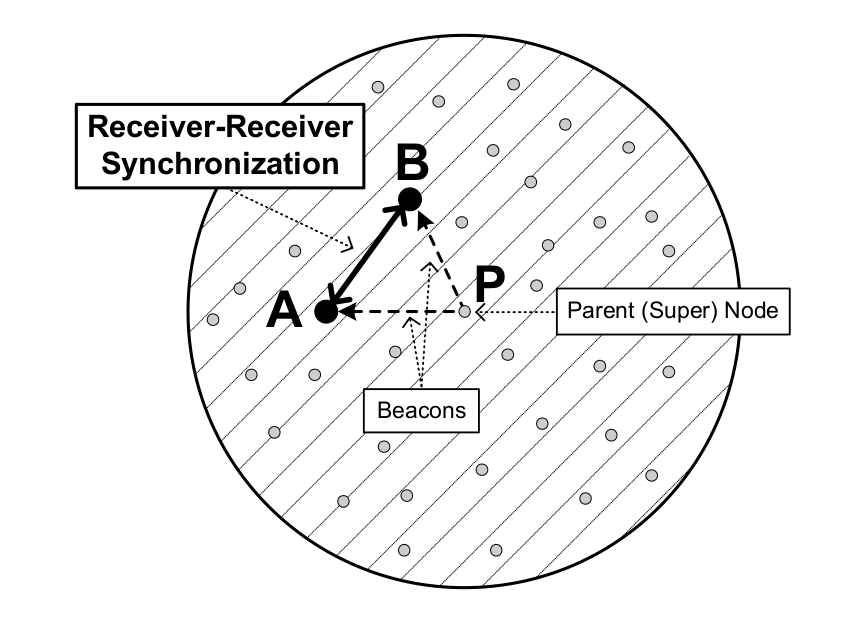
\includegraphics[scale=0.5,width=15cm,height=9cm]{photos/receiver_receiver.png}
	    	\caption{Receiver-receiver synchronizatio}
	    	\label{fig:x Receiver_to_receiver}
	    	
	    \end{figure}
    
    
    
    \subsection{Receiver only synchronization}
	    A group of nodes can be simultaneously synchronized by only listening to the message exchanges of a pair of nodes\cite{book} see\ref{fig:x Receiver_Only}.
	    %figure
	    \begin{figure}[h!]
	    	\centering
	    	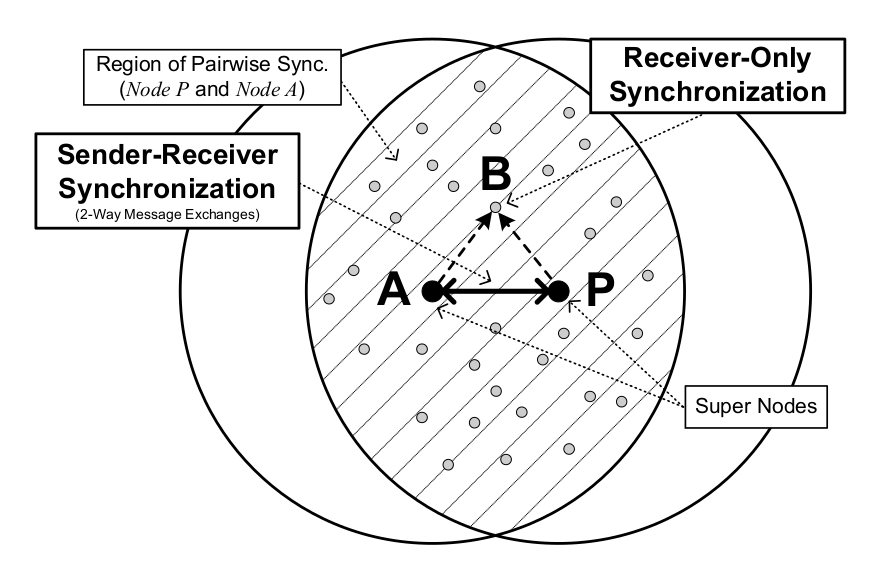
\includegraphics[scale=0.5,width=15cm,height=9cm]{photos/reciverOnly.png}
	    	\caption{Receiver-only synchronization}
	    	\label{fig:x Receiver_Only}
	    	
	    \end{figure}
	    
    
    
    
\section{Time Synchronization Protocols}
A time synchronization protocol should be able to work optimally in terms of all the design requirements imposed on time synchronization in WSNs\cite{book}, which include energy efficiency, scalability, precision, security, reliability, and robustness to network dynamics. However, the complex nature of WSNs makes it very difficult to optimize the protocol with respect to all these requirements simultaneously\cite{book}. Due to the tradeoffs in satisfying these requirements, each protocol is designed to put distinct emphases on different requirements\cite{book}.
\newline Time synchronization protocols can be categorized into following classes :\cite{book}
\begin{itemize}
	\item Master–slave vs. peer-to-peer : 
	\item Clock correcting vs. untethered clock :
	\item Synchronization approach : 
	\item Pairwise synchronization vs. network-wide synchronization :
\end{itemize}


\subsection{Lightweight Tree-Based Synchronization}
The primary goal of the Lightweight Tree-Based Synchronization (LTS) protocol (VanGreunen and Rabaey 2003) is to provide a specified precision (instead of a maximum precision) with as little overhead as possible. LTS can be used with different algorithms for both centralized and decentralized multi-hop synchronization.

\subsection{Timing-sync Protocol for Sensor Networks}
The Timing-sync Protocol for Sensor Networks (TPSN) (Ganeriwal et al. 2003) is another traditional sender–receiver synchronization approach that uses a tree to organize a network. TPSN uses two phases for synchronization: the level discovery phase (executed
during network deployment) and the synchronization phase.
\subsection{Flooding Time Synchronization Protocol}
The goals of the Flooding Time Synchronization Protocol (FTSP) (Maróti et al. 2004) are
to achieve network-wide synchronization with errors in the microsecond range, scalability
up to hundreds of nodes, and robustness to changes in network topology including link
and node failures. FTSP differs from other solutions in that it uses a single broadcast
to establish synchronization points between sender and receivers while eliminating most
sources of synchronization error
\subsection{Consensus-based Multi-hop Time	Synchronization Protocol in Wireless Sensor	Networks}
The Consensus Time Synchronization \cite{sync2} is a novel distributed time synchronization approach which overcomes the shortcomings of centralized and consensus time synchronization schemes by combining their advantages. The timing messages are exchanged following the RO methodology. This reduces the communication overhead and energy consumption and speeds up the convergence time. The sensor nodes compensate their clock offset and skew by synchronizing to multiple synchronized nodes which increases synchronization accuracy and robustness to node failures. In addition, nodes are organized intohierarchical structure, which allows to establish a particular communication pattern between nodes leading to reduce the number of exchanged messages and the convergence time .



	
	\chapter{Conception}
	\section{Introduction}
In all modern (High Level) programming language , You will find one or more library that deals with big numbers , that because the pure language types don't support big number types and arbitrary precision arithmetic on integers , This because hardware limitation , so developers have tried to make libraries that emulate hardware on top of software so they can provide operation on number with big number of digits .\newline

Exemples : 
 \begin{itemize}
	\item The GNU MP Bignum C-Library
	\item The Boost C++ Library (arbitrary precision lib)
\end{itemize}

The two libraries above are the main libs which are used and have a big community around them in c/c++ based programs ,But the problem these is that this two libraries can't be run on a device like raspberry or an adruino bacause of memory limitation ,and like most other motes used in wireless sensor network are c-based and has low memory, so All these kinda devices need a tiny library that has just main and base arithmetic operations in order to run and compute some operation that has numbers with big digits .
\section{Main Idea}
The main idea of representing big numbers structure is to define a data structure (Discussed in Data Structures section) that is composed of two arrays of fixed size which will hold the integer part,fractional part respectively ,define sign bit which will be holding the sign of the number all time ,and also defining an integer number which will be holding the digits' number of integer part to be able to keep tracking of the integer part.Then lastly define all basic arithmetic operation(Discussed in algorithms section) on this data structure like addition,substraction,multiplication and division algorithms .
\section{Library structure}
The main benefits of this library is that it doesn't has any dynamic allocation at all , instead it has a configuration file that you must initialize some macros on it in order precise the maximum number of digits that you're expecting to use for two Integer,Floating parts before compilation time ,so it will let heap space for the other important works that must be done in real time . 

\subsection{Data Structures}
In this section we will be describing the main data structure that will be used in this library 
\begin{center}
	\line(1,0){250}
\end{center}
\paragraph{bnstruct} is the main data structure that will hold all big numbers through this library :
\begin{lstlisting}[style=CStyle]
	struct bnstruct{
	 char intNum[MaxInt+1];
	 char floatNum[MaxFloat+1];
	 unsigned short intlen;
	 bool signNum;
	
	};
	
	typedef struct bnstruct bn;
\end{lstlisting}

\begin{itemize}
	\item char intNum : This is a char array that will holds the integer part of the big number.
	\item MaxInt : This is a macro that hold the maximum number of digits in decimal part that bn structure will support in run time. 
	\item char floatNum : This is a char array that will holds the rational part of the big number .
	\item MaxFloat : This is a macro that hold the maximum number of digits in decimal part that bn structure will support in run time.
	\item unsinged short intlen : a positive short number that will holds the length of the decimal part.
	\item bool signNum : a boolean number that will holds the sign of the big number(Positive,Negative).
\end{itemize}
\begin{center}
	\line(1,0){250}
\end{center}
\paragraph{splittedNum} is the main data structure that will hold all big numbers that are splitted into two bignumbers through this library :\newline\newline
Exemple : 
\begin{itemize}
	\item Original number($a_{n},a_{n-1},...,a_{0}$)
	\item Splitted Number($a_{j-1},a_{j-2},...,a_{0}$ $|$ $a_{n},a_{n-1},...,a_{j}$ $|$ $10^{j}$)
\end{itemize}





 

\begin{lstlisting}[style=CStyle]
struct splittedNum{
	bn first;
	bn second;
	unsigned int shift;
};
\end{lstlisting}

\begin{itemize}
	\item bn first : This structure will hold the first part of the original big number 
	\item bn second : This structure will hold the first part of the original big number
	\item unsigned int shift : this integer will hold the length of the decimal part of first number
\end{itemize}



\subsection{Algorithmes}
This library has the implementation of the main algorithmes to provide the main arithmetic operations on big number structure that was described above . In this section we'll be describing these algorithmes .



%%addition algorithme

\newpage
\begin{center}
	\line(1,0){250}
\end{center}

\paragraph{Addition Algorithm}
This algorithm is used as main and basic operation for adding see(Addition Algorithm) to big numbers ,it takes two big numbers as an input then returns the addition .It has linear time complexity O(n) where n is equal to summation of integer part length,fractional part length respectively . 
\newline\newline\newline\newline\newline\newline\newline\newline\newline
\begin{algorithm}[H]
	\SetAlgoLined
	\KwIn{$num1(n1d_{MaxInt},...,n1d_{0}$ $ . $  $n1f_{MaxFloat},...,n1f_{0}) $
		
		\hspace{1.25cm}$  num2(rd_{MaxInt},...,rd_{0}$ $ . $  $ n2f_{MaxFloat},...,n2f_{0})$}
	\KwResult{$result(rd_{MaxInt},...,rd_{0}$ $ . $  $rf_{MaxFloat},...,rf_{0})$ }
	i,carry = 0,tmp=0\;

	\For{i in $range(MaxFloat,0)$}
	{
		
		$tmp = (n1f_{i} + n1f_{i} + carry);$
		
		$rf_{i} =  tmp $\%$ 10;$ 
		
		$carry = tmp $/$ 10;$
	}

		\For{i in $range(MaxInt,0)$}
	{
		
		$tmp = (n1d_{i} + n1d_{i} + carry);$
		
		$rd_{i} =  tmp $\%$ 10;$ 
		
		$carry = tmp $/$ 10;$
	}
	\caption{Addition}
	\label{Addition_Algorithm}
\end{algorithm}



%%substraction algorithm
\newpage
\begin{center}
	\line(1,0){250}
\end{center}

\paragraph{Substraction Algorithm}
This algorithm is used as main and basic operation for substracting see(Substraction Algorithm) to big numbers ,it takes two big numbers as an input then returns the substraction .It has linear time complexity O(n) where n is equal to summation of integer part length,fractional part length respectively . 
\newline\newline\newline\newline\newline\newline\newline\newline\newline
\begin{algorithm}[H]
	\SetAlgoLined
	\KwIn{$num1(n1d_{MaxInt},...,n1d_{0}$ $ . $  $n1f_{MaxFloat},...,n1f_{0}) $
		
		\hspace{1.25cm}$  num2(rd_{MaxInt},...,rd_{0}$ $ . $  $ n2f_{MaxFloat},...,n2f_{0})$}
	\KwResult{$result(rd_{MaxInt},...,rd_{0}$ $ . $  $rf_{MaxFloat},...,rf_{0})$ }
	i,borrow = 0,tmp=0\;
	
	\For{i in $range(MaxFloat,0)$}
	{
		
		$tmp = (n1f_{i} - n1f_{i} - carry);$
		
		
 	 	 \eIf{$tmp < 0$}
 	 	 {
  	 	 	$tmp += 10;$
  	 	 
  	 	    $borrow = 1;$
   	 	}
 	 	{
  			$borrow  = 0;$
		}
		$rf_{i} =  tmp;$ 
		
	}
	
	\For{i in $range(MaxInt,0)$}
	{
			$tmp = (n1d_{i} - n1d_{i} - borrow);$
		
		
		\eIf{$tmp < 0$}
		{
			$tmp += 10;$
			
			$borrow = 1;$
		}
		{
			$borrow  = 0;$
		}
		$rd_{i} =  tmp;$ 
	
	}
	\caption{Substraction}
	\label{substraction_algorithm}
\end{algorithm}



%%Multiplication algorithm
\newpage
\begin{center}
	\line(1,0){250}
\end{center}
\paragraph{Multiplication Algorithm}
This algorithm is used as main and basic operation for multiplication see(Multiplication Algorithm) to big numbers ,it takes two big numbers as an input then returns the multiplication .It has linear time complexity O($n^{1.59}$) where n is equal to maximum of integer part length,fractional part length respectively .
\newline\newline\newline\newline\newline\newline\newline\newline\newline
\begin{algorithm}[H]
	\SetAlgoLined
	\KwIn{$num1(n1d_{MaxInt},...,n1d_{0}$ $ . $  $n1f_{MaxFloat},...,n1f_{0}) $
		
		\hspace{1.25cm}$  num2(rd_{MaxInt},...,rd_{0}$ $ . $  $ n2f_{MaxFloat},...,n2f_{0})$}
	\KwResult{$result(rd_{MaxInt},...,rd_{0}$ $ . $  $rf_{MaxFloat},...,rf_{0})$ }
	s1 = 0,s2 = 0,tmp1,tmp2,tmp3,tmp4;

	\eIf{num1 is equal to Zero or num2 is equal to zero}
	{
		$result = Zero;$
	}
	
	\eIf{both num1 and num2 are simple numbers}
	{
		$result = num1 * num2;$ 
	}
	{
		\eIf{num1 is simple and num2 is big number}
		{
			$splitNum(num2,tmp1,tmp2,s1);$
			
			$result = addition(multiplication(num2,tmp1),sh10(multiplication(num2,tmp2),s1));$	
		}
		{
				\eIf{num2 is simple and num1 is big number}
				{
						$splitNum(num1,tmp3,tmp4,s2);$
					
						$result = addition(multiplication(num1,tmp3),sh10(multiplication(num1,tmp4),s2));$
			
				}
				{
					% (tmp1+tmp22*shift1)*(tmp3+tmp4*shift2)
					$splitNum(num1,tmp1,tmp2,s);$
					
					$splitNum(num2,tmp3,tmp4,s2);$
					$result = add(mul(tmp1,tmp3),sh10(mul(tmp1,tmp4),s2),sh10(mult(tmp2,tmp3),s1),$
					$sh10(mul(tmp2,tmp4),s1+s2));$
				
				}
	
		}	
	
	}

	\caption{Multiplication}
	\label{multiplication_Algorithm}
\end{algorithm}



%%Division algorithm
\newpage
\begin{center}
	\line(1,0){250}
\end{center}

\paragraph{Division Algorithm}
This algorithm is used as main and basic operation for Division see(Division Algorithm) to big numbers ,it takes two big numbers as an input then returns the disivion .It has linear time complexity O(n) where n is equal to summation of integer part length,fractional part length respectively .
\newline\newline\newline\newline\newline\newline\newline\newline\newline


\begin{algorithm}[H]
	\SetAlgoLined
	\KwIn{$num1(n1d_{MaxInt},...,n1d_{0}$ $ . $  $n1f_{MaxFloat},...,n1f_{0}) $
		
		\hspace{1.25cm}$  num2(rd_{MaxInt},...,rd_{0}$ $ . $  $ n2f_{MaxFloat},...,n2f_{0})$}
	\KwResult{$result(rd_{MaxInt},...,rd_{0}$ $ . $  $rf_{MaxFloat},...,rf_{0})$ }
	idx = 0,tmp=0,shift1,shift2;
	\eIf{num2 is equal to Zero}
	{
		Division can't be done;
	}
	{
		\eIf{num1 is equal to Zero}
		{
			$result = Zero;$
		}
		{
			1 - shift num1,num2 till there's no float digit and put the shift in shift1,shift2 respectively;
		
			$tmp  = n1d_{idx}$

		%	\whiledo{$tmp is less than num2$}
		%	{
			%%	$temp = temp * 10 +(n1d_{idx++};$
		%	} 
			
		%	\whiledo{$idx is less than the length of num1$}
		%	{
			%%	$temp = temp * 10 +(n1d_{idx++};$
				
			%%	$addition(result,tmp/num2);$
				
			%%	$ temp = (temp \% divisor) * 10 + $$number_{idx++};$
		%	} 
			
		
		}	

	}
	

	\caption{Division}
	\label{division_algorithm}
\end{algorithm}


\newpage
\subsection{Interfaces}
In this section we will be describing main interfaces that library's user will interact with them .

%void uadd(bn,bn,bn*);
\paragraph{void uadd(bn,bn,bn*)} This interface does unsigned addition on big number , It doesn't care about sign of the first two parameters and it return always a positive number in third parameter
$$Usage : uadd(@arg1,@arg2,@resultOfAddition)  $$ 

%void usub(bn,bn,bn*);

\paragraph{void usub(bn,bn,bn*)} This interface does unsigned substraction on big number , It doesn't care about sign of the first two parameters and it return always a positive number in third parameter
$$Usage : usub(@arg1,@arg2,@resultOfSubstraction)  $$ 
%void umul(bn,bn,bn*);


\paragraph{void usub(bn,bn,bn*)} This interface does unsigned multiplication on big number , It doesn't care about sign of the first two parameters and it return always a positive number in third parameter
$$Usage : umul(@arg1,@arg2,@resultOfMultiplication)  $$ 

%void bc_divide(bn,bn,bn*);

\paragraph{void ubc\_divide(bn,bn,bn*)} This interface does unsigned division on big number , It doesn't care about sign of the first two parameters and it return always a positive number in third parameter
$$Usage : ubc\_divide(@arg1,@arg2,@resultOfDivision)  $$ 





%void add(bn,bn,bn*);
%void uadd(bn,bn,bn*);
\paragraph{void add(bn,bn,bn*)} This interface does signed addition on big number .
$$Usage : add(@arg1,@arg2,@resultOfAddition)  $$ 

%void usub(bn,bn,bn*);

\paragraph{void sub(bn,bn,bn*)} This interface does signed substraction on big number .
$$Usage : sub(@arg1,@arg2,@resultOfSubstraction)  $$ 
%void umul(bn,bn,bn*);


\paragraph{void mul(bn,bn,bn*)} This interface does signed multiplication on big number .
$$Usage : mul(@arg1,@arg2,@resultOfMultiplication)  $$ 

%void bc_divide(bn,bn,bn*);

\paragraph{void bc\_divide(bn,bn,bn*)} This interface does signed division on big number .
$$Usage : bc\_divide(@arg1,@arg2,@resultOfDivision)  $$ 


	
	\chapter{Results}
	In this chapter we will be discussion and showing different results that were obtained while doing simulation and experimentation in both real devices and emulation .

\section{Clock Estimators}

 $$a_{i} = \frac{S \sum^{J_{i}}_{j=1}(\sum^{K_{j}}_{k=1}t_{jK}^{i}.t^{i}_{j}) - \sum^{J_{i}}_{j=1}(\sum^{K_{j}}_{k=1}(t_{jK}^{i})) * \sum^{K_{J_{i}}}_{i=1}(t_{j}^{i}* k_{i})}{S \sum^{J_{i}}_{j=1}(\sum^{K_{j}}_{K=1} (t_{i}^{j})^{2}) - (\sum_{j=1}^{J_{i}}(\sum^{K_{j}}_{K=1} t_{i}^{j}))}
         $$


$$ b_{i} =  \frac{1}{S} [ \sum_{j=1}^{J_{i}}(\sum_{K=1}^{K_{j}} t_{j_{k}}^{i}) - a_{i} * \sum_{j=1}^{J_{i}}(\sum_{K=1}^{K_{j}}t_{j}^{i}.K_{i}) ]$$
\section{Programming Language}
\subsection{C}
C is a general-purpose, imperative computer programming language, supporting structured programming, lexical variable scope and recursion, while a static type system prevents many unintended operations.
\section{Tools}
\subsection{Clion}
Smart C and C++ editor,Thanks to native C and C++ support, including modern C++ standards, libc++ and Boost, CLion knows your code through and through and takes care of the routine while you focus on the important things.
\subsection{Cmake}
CMake is a cross-platform free and open-source software for managing the build process of software using a compiler-independent method. It supports directory hierarchies and applications that depend on multiple libraries.
\subsection{Git}
Git is a free and open source distributed version control system designed to handle everything from small to very large projects with speed and efficiency. Git is easy to learn and has a tiny footprint with lightning fast performance.

\section{Devices}
\subsection{Raspberry}
A Raspberry Pi is a credit card-sized computer originally designed for education, inspired by the 1981 BBC Micro. Creator Eben Upton's goal was to create a low-cost device that would improve programming skills and hardware understanding at the pre-university level.
\subsection{Arduino}
Arduino is an open source computer hardware and software company, project, and user community that designs and manufactures single-board microcontrollers and microcontroller kits for building digital devices and interactive objects that can sense and control objects in the physical and digital world
\section{Emulator}
\subsection{Qemu}
QEMU is a generic and open source machine emulator and virtualizer. Screenshot: QEMU running the ReactOS operating system on Linux. Full-system emulation. Run operating systems for any machine, on any supported architecture.


\section{Basic Arithmetic Operations Timing}
In this section we will be showing time consumation for the basic arithmetic operations depending on the number of digits of operands .

\section{Estimator Calculation Timing}
In this section we will be showing time consumation for calculating the estimator in function of number length
\begin{figure} 
   % \subsection{Raspberry result}

	\hfill
	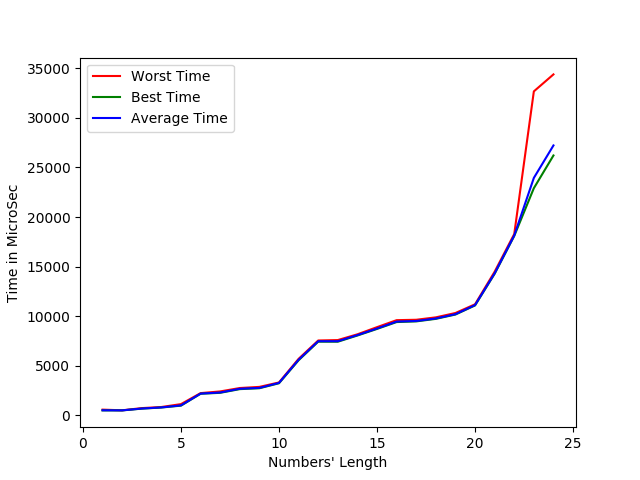
\includegraphics[scale=0.5,width=12cm,height=5cm]{result/raspberry_res.png}
	\caption{Raspberry estimator calculation time}
	\centering
	\label{fig:x raspberry_res}
	\hspace*{\fill}
\end{figure}

\begin{figure} 
   % \subsection{arduino result}

	\hfill
	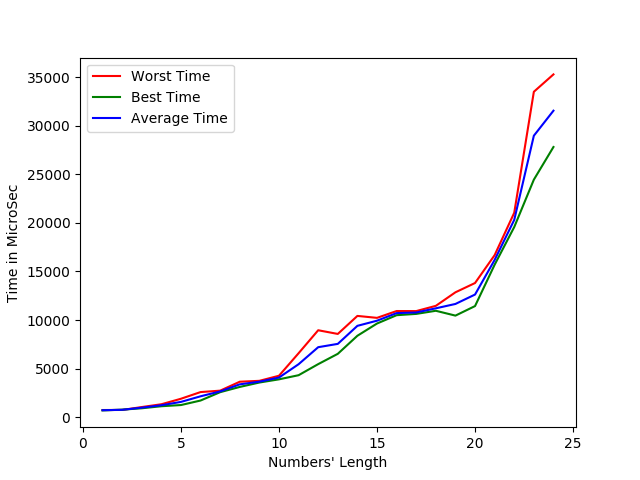
\includegraphics[scale=0.5,width=12cm,height=5cm]{result/arduino_res.png}
	\caption{Arduino estimator calculation time}
	\centering
	\label{fig:x arduino_res}
	\hspace*{\fill}
\end{figure}

\begin{figure} 
   % \subsection{pc result}

	\hfill
	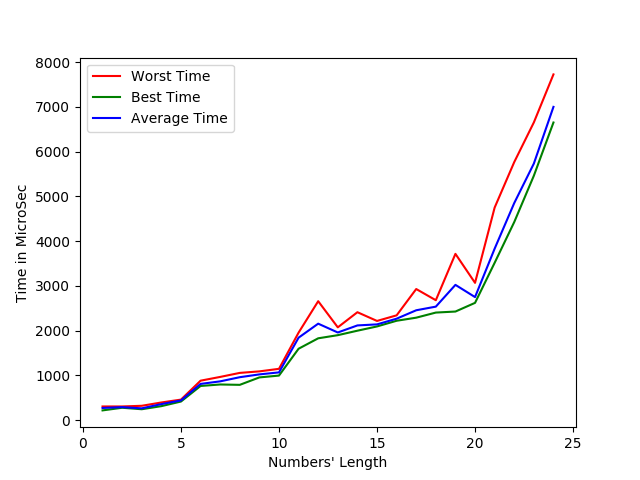
\includegraphics[scale=0.5,width=12cm,height=5cm]{result/pc_res.png}
	\caption{Pc estimator calculation time}
	\centering
	\label{fig:x pc_res}
	\hspace*{\fill}
\end{figure}
	\printbibliography
\end{document}
	

	
